%
% File: chap01.tex
%
\let\textcircled=\pgftextcircled
\chapter{Flux in the core}
\label{chap:intro}

\initial{S}everal exercises from the book written by M. M. El Wakil~\cite{book01} are tackled in this homework. The problems in this section relate to the second chapter of the book, covering the subject of the neutrons and their interactions.

%=======
\section{Finite cylinder}
\label{prob31}

\subsection{Problem}
\textit{Find the flux in a finite cylinder of radius $R$ and height $H$ using the diffusion theory.}

\subsection{Solution}

The diffusion equation can be written following Equation~\ref{eq31}.

\begin{equation}\label{eq31}
\nabla^2 \phi + B^2\phi = 0
\end{equation}

In a cylindrical coordinates system, the Laplacian $\nabla$ can be explicited according to Equation~\ref{eq32}.

\begin{equation}\label{eq32}
\nabla^2 \phi = \frac{\partial^2}{\partial r^2} + \frac{1}{r}\frac{\partial}{\partial r} + \frac{\partial^2}{\partial z^2}
\end{equation}

Consequently, we can rewrite Equation~\ref{eq31} to obtain Equation~\ref{eq33}.


\begin{equation}\label{eq33}
\frac{\partial^2 \phi(r, z)}{\partial r^2} + \frac{1}{r}\frac{\partial \phi(r, z)}{\partial r} + \frac{\partial^2 \phi(r, z)}{\partial z^2} + B^2\phi(r, z) = 0
\end{equation}

In order to solve this differential equation, one assumes that the axial flux component is independent from the radial flux component. In this case, the variables can be separated, using Definition~\ref{eq34}.


\begin{equation}\label{eq34}
\phi(r, z) = \rho(r)\zeta(z)
\end{equation}

This implies Equation~\ref{eq35}.


\begin{equation}\label{eq35}
\zeta(z)\frac{\partial^2 \rho(r)}{\partial r^2} + \frac{\zeta(z)}{r}\frac{\partial \rho(r)}{\partial r} + \rho(r)\frac{\partial^2 \zeta(z)}{\partial z^2} + B^2\rho(r)\zeta(z) = 0
\end{equation}

Now, it is useful to divide the equation by $\rho(r)\zeta(z)$ in order to isolate the $r$-component from the $z$-component, as seen in Equation~\ref{eq36}.


\begin{equation}\label{eq36}
\frac{1}{\rho(r)}\frac{\partial^2 \rho(r)}{\partial r^2} + \frac{1}{r\rho(r)}\frac{\partial \rho(r)}{\partial r} + \frac{1}{\zeta(z)}\frac{\partial^2 \zeta(z)}{\partial z^2} = -B^2
\end{equation}

Now, we have an equation of the form $f(x) + g(y) = cst$. This equation can only be verified if $f(x) = cst$ and $g(y) = cst$. Consequently, we have the following system of equations~\ref{eq37} and~\ref{eq38} to solve.

\begin{alignat}{2}
\frac{1}{\rho(r)}\frac{\partial^2 \rho(r)}{\partial r^2} + \frac{1}{r\rho(r)}\frac{\partial \rho(r)}{\partial r} = -\alpha \label{eq37} \\     \frac{1}{\zeta(z)}\frac{\partial^2 \zeta(z)}{\partial z^2} = -\beta \label{eq38}
\end{alignat}

Where:

\begin{conditions}
\alpha + \beta & $B^2$
\end{conditions}

Focusing on Equation~\ref{eq37} first, one can multiply both sides by $\rho(r)$, obtaining Equation~\ref{eq39}.

\begin{equation}\label{eq39}
\frac{\partial^2 \rho(r)}{\partial r^2} + \frac{1}{r}\frac{\partial \rho(r)}{\partial r} + \alpha\rho(r) = 0
\end{equation}

Equation~\ref{eq39} is known as a Bessel equation. The solutions to this equation are the first and second kind of Bessel functions, $J_0(\sqrt{\alpha}r)$ (Figure~\ref{fig31}) and $Y_0(\sqrt{\alpha}r)$ (Figure~\ref{fig32}).

\begin{figure}[t!]
	\centering
	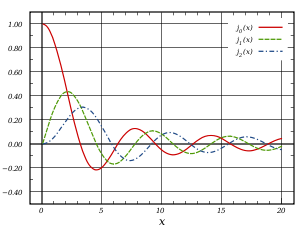
\includegraphics[height=0.3\textheight]{fig/bessel_j.png}
	\mycaption[Bessel function of the first kind - $J$]{Bessel function of the first kind - $J$.}
	\label{fig31}
\end{figure}


\begin{figure}[t!]
	\centering
	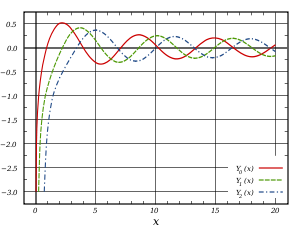
\includegraphics[height=0.3\textheight]{fig/bessel_y.png}
	\mycaption[Bessel function of the second kind - $Y$]{Bessel function of the second kind - $Y$.}
	\label{fig32}
\end{figure}

Consequently, the solution will be of the form $\rho(r) = AJ_0(\sqrt{\alpha}r) + CY_0(\sqrt{\alpha}r)$, $A$ and $C$ being constants.

We can now use boundary conditions. We know that the radial component of the flux has to be greater or equal to 0 $\forall r$. In our system, r = 0 at the center of the cylinder. However, $\lim_{r\to 0} Y_0(r) = -\infty$, implying that $C = 0$.

We also know that at a radius $R_e = R + \delta_e$, the flux is to be zero. Thus, $\phi(R_e) = 0$. So, we have to solve Equation~\ref{eq310}.

\begin{equation}\label{eq310}
AJ_0(\sqrt{\alpha}R_e) = 0
\end{equation}

This can be solved by A = 0, in which case we would obtain the trivial solution $\rho(r) = 0$, of no interest. $J_0(x) = 0$ can be verified for several $x$. However, since the flux has to be positive, the solution has to be the first zero of the function, happening for $x = 2.405$. Hence, Equation~\ref{eq310} is verified for $\sqrt{\alpha}R_e = 2.405$.

Thus, we have the solution of the radial component of the flux, presented in Equation~\ref{eq311}.

\begin{equation}\label{eq311}
\rho(r) = AJ_0(\frac{2.405}{R_e}r)
\end{equation}

Now, we can focus on the axial component of the flux, shown in Equation~\ref{eq38}. It is interesting to recognize in this equation the equation for an infinite slab geometry, for which the solution is known, explicited in Equation~\ref{eq312}.

\begin{equation}\label{eq312}
\zeta(z) = D\cos(\frac{\pi}{H_e}z)
\end{equation}

Finally, one can compute the flux $\phi(r, z)$, according to Equation~\ref{eq34}.

\begin{equation}\label{eq312}
\phi(r, z) = \phi_0 * J_0(\frac{2.405}{R_e}r)\cos(\frac{\pi}{H_e}z)
\end{equation}

Where $\phi_0 = A * D$.

We can also deduce the buckling $B^2 = \alpha + \beta = \left( \frac{2.405}{R_e} \right)^2 + \left( \frac{\pi}{H_e} \right)^2$.
